\documentclass[pstricks,border=11pt]{article}

\hfuzz=0.64pt

\usepackage[utf8]{inputenc}

\usepackage{graphicx}
\graphicspath{ {./images/} }
\usepackage{amsmath} % for the equation* environment
\usepackage{tabularx}
\usepackage{multirow} % Required for multirows
\usepackage{booktabs} % For prettier tables
\usepackage{siunitx} % Required for alignment
\usepackage{pgfplots}
\usepackage{pst-plot}
\usepackage{hyperref}

\pgfplotsset{compat = newest}
\sisetup{
  round-mode          = places, % Rounds numbers
  round-precision     = 2, % to 2 places
}

\title{EECS Exam 4 Study Guide}
\author{Tiffany Pham}
\date{26 April 2023}

\begin{document}

\maketitle

\section{Topics}
The last exam for the semester will be on \textbf{Tuesday, May 2nd}. The following will be covered:
\begin{itemize}
    \item \textit{Make: Electronics 3rd ed.} Experiments 23 (Nice Dice) and 30 (Nicer Dice)
    \item The reading about Claude Shannon and Information Theory
    \item Your assigned chip. Know the following about your chip:
    \begin{itemize}
        \item []The pinout diagram and function of each pin
        \item []Current and voltage requirements and limitations
        \item []A simple test circuit that can verify the chip is working properly
        \item []Examples of practical applications for the chip
    \end{itemize}
\end{itemize}

\section{4017 Chip}
What does the 4017 chip do?
\hfill \break
The CD4017 IC is a CMOS Decade counter and it is used in the applications of low-range counting. This IC will count from 0 to 10 and the circuit with an IC 4017 will save board space as well as the time necessary to design the circuit. This decade counter is similar to Johnson 10 stage decade counter. This CMOS IC is frequently used in designing the 10 LEDs-based circuits to run the light for beginners. So it is one of the most flexible counters because it counts up to 10 \& also it includes 10 separate outputs. This IC includes the counter as well as the decoder.

\hfill \break
\subsection{Picture Layout:}

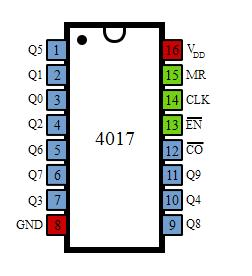
\includegraphics[scale=1]{IC-4017-Pin-Diagram.jpeg}
\hfill \break
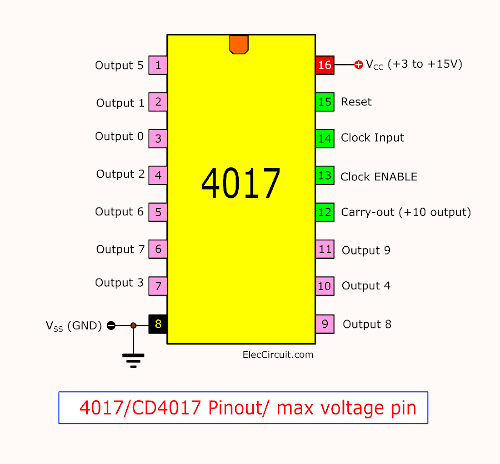
\includegraphics[scale=.5]{images/CD4017-pinout.png}
\hfill \break
\vspace{15mm}

\subsection{Explanation of what each pin does:}
It has 16 pins and the functionality of each pin is explained as follows:
\begin{itemize}
    \item Pin-1: It is the output 5. It goes high when the counter reads 5 counts.
    \item Pin-2: It is the output 1. It goes high when the counter reads 0 counts.
    \item Pin-3: It is the output 0. It goes high when the counter reads 0 counts.
    \item Pin-4: It is the output 2. It goes high when the counter reads 2 counts.
    \item Pin-5: It is the output 6. It goes high when the counter reads 6 counts.
    \item Pin-6: It is the output 7. It goes high when the counter reads 7 counts.
    \item Pin-7: It is the output 3. It goes high when the counter reads 3 counts.
    \item Pin-8: It is the Ground pin that should be connected to a LOW voltage (0V).
    \item Pin-9: It is the output 8. It goes high when the counter reads 8 counts.
    \item Pin-10: It is the output 4. It goes high when the counter reads 4 counts.
    \item Pin-11: It is the output 9. It goes high when the counter reads 9 counts.
    \item Pin-12: This is divided by 10 output which is used to cascade the IC with another counter to enable counting greater than the range supported by a single IC 4017. By cascading with another 4017 IC, we can count up to 20 numbers. We can increase and increase the range of counting by cascading it with more and more IC 4017s. Each additional cascaded IC will increase the counting range by 10. However, it is not advisable to cascade more than 3 ICs as it may reduce the reliability of the count due to the occurrence of glitches. If you need a counting range of more than twenty or thirty, I advise you to go with the conventional procedure of using a binary counter followed by a corresponding decoder.
    \item Pin-13: This pin is the disabled pin. In the normal mode of operation, this is connected to ground or logic LOW voltage. If this pin is connected to logic HIGH voltage, then the circuit will stop receiving pulses and so it will not advance the count irrespective of several pulses received from the clock.
    \item Pin-14: This pin is the clock input. This is the pin from where we need to give the input clock pulses to the IC to advance the count. The count advances on the rising edge of the clock.
    \item Pin-15: This is the reset pin that should be kept LOW for normal operation. If you need to reset the IC, then you can connect this pin to HIGH voltage.
    \item Pin-16: This is the power supply (Vcc) pin. This should be given a HIGH voltage of 3V to 15V for the IC to function.
\end{itemize}

\subsection{Features and specifications}
The main features and specifications of IC 407 include the following.
\begin{itemize}
    \item The supply voltage of IC 4017 ranges from 3V to 15V, usually +5V
    \item This IC is well-matched with Transistor-Transistor Logic or TTL.
    \item The operational speed/CLK speed of this IC is 5 MHz.
    \item It provides support to 10 outputs that are decoded.
    \item It is available in different packages like 16-pin GDIP, PDIP \& PDSO
    \item Input high time 30 ns
    \item Output current is 10 mA
    \item Noise immunity is high typically 0.45 VDD
    \item Operation is completely static
    \item Low power like 10 µW
    \item Speed operation is medium like 5.0 MHz with 10V VDD
    \item Input Voltage or Vin ranges from $-$0.5 VDC to VDD $+$0.5 VDC
    \item TS or Storage Temperature ranges from $-$65°C to $+$150°C
    \item VDD or DC Supply Voltage ranges from $-$0.5 VDC to $+$18 VDC
    \item PD or Power Dissipation is Dual-In-Line is 700 mW
    \item TL or Lead Temperature is 260°C
\end{itemize}
\hfill \break
In various electronic circuit applications, this IC 4017 decade counter is one of the most versatile and useful chips. Practically, it is also known as “Johnson 10 stage decade counter divider. Here the 10 number is connected through the number of o/ps this counter has that will turn into high in series in reply to each high CLK pulse that is given at its input CLK pinout. This means, all its outputs will use a single cycle of high o/p sequencing from beginning to end in reply to 10 CLKs and it is received at its input. As the name suggests, so it is counting in a way \& also separating the input CLK through 10.

\subsection{Examples of practical applications for the chip}
The applications of IC CD4017 include the following:
\begin{itemize}
    \item The most popular IC like CD4017 is extensively used in different applications which includes Decoder, Binary counter, Frequency division, Decade counter, etc. Additionally, this IC is also used to make different electronics projects like Remote controlled Switch, Light Chaser, Touch ON-OFF switch, Alarm, Matrix Die, Clap switch, etc.
    \item This decade counter IC can also be used in different industries like automotive, alarms, electronic manufacturing of medical instruments \& instrumentation devices.
    \item This IC is used in counting applications which can switch ON 10 outputs in sequence within a fixed time \& reset the count otherwise hold it once necessary. It also indicates the counting status through the Carry pin that is used in LED chasers as well as other logical output projects. So this IC is the best choice if you are searching for a sequential decoded counting IC to count up to 10
\end{itemize}

\hfill \break
\section{Experiment 23: Nice Dice}
\begin{enumerate}
    \item What is a decade counter?
    \begin{itemize}
        \item A decade counter counts in decimal digits, rather than binary. A decade counter may have each (that is, it may count in binary-coded decimal, as the 7490 integrated circuit did) or other binary encodings. A decade counter is a binary counter designed to count to 1001 (decimal 9). And it resets for every new clock input. As it can go through 10 unique combinations of output, it is also called as “Decade counter”.
    \end{itemize}
    \item How many counters are in the "393" chip?
    \begin{itemize}
        \item Two counters
    \end{itemize}
    \item How many outputs are available (bits, or binary digits) are available per counter on the "393?"
    \begin{itemize}
        \item It has two counters, each with 4-bit outputs on pins labeled A, B, C, and D. So technically 8 outputs.
    \end{itemize}
    \item How high can one of the counters on the "393" count?
    \begin{itemize}
        \item It can count to 1.
    \end{itemize}
    \item What if you used one counter to run the other on the chip? How high could it count?
    \begin{itemize}
        \item aaaa
    \end{itemize}
    \item What is meant by the "modulus" of a counter?
    \begin{itemize}
        \item It is the highest number of pulses that a counter reaches before it repeats.
    \end{itemize}
    \item It's easy to run the counter on modulus, 2, 4, 8, or 16. How can we get the "393" chip to do modulus 6? \textbf{(ALL FOUND ON Page 221)}
    \begin{itemize}
        \item You can stick an AND gate in. You can use logic chip(s) with a counter to change the modulus of the counter by looking for a distinctive pattern in the output states and feeding back a signal to the reset pin.
    \end{itemize}
    \item Does the "Nice Dice" circuit produce an intrinsically random number?
    \begin{itemize}
        \item Yes
    \end{itemize}
\end{enumerate}


\section{Experiment 30: Nicer Dice}
\begin{enumerate}
    \item Why is it difficult to truly generate a random number?
    \begin{itemize}
        \item Randomness is relational. The problem modern computers have with randomness is that it doesn't make mathematical sense. You can't program a computer to produce true randomness—wherein no element has any consistent, rule-based relationship to any other element—because then it wouldn't be random. "A random number is basically something that a device produces, and we cannot know its value until it has been generated." "One of the most difficult parts of generating random numbers is basically that a computer is a machine that repeats a few steps we tell it to do, it cannot generate them.
    \end{itemize}
    \item What is pseudo-code?
    \begin{itemize}
        \item In computer science, pseudocode is a plain language description of the steps in an algorithm or another system. Pseudocode often uses structural conventions of a normal programming language, but is intended for human reading rather than machine reading. Pseudocode is a simplified representation of an algorithm that uses the English language to describe coding logic. It allows programmers to plan any algorithm's structure using simple commands. Pseudocode primarily uses plain text to describe various coding actions and their correct sequence in the algorithm.
    \end{itemize}
    \item What do you feel is more random, this process, or the 74HC393/555-based dice from Experiment 23?
    \begin{itemize}
        \item I don't really know. I feel like both of them are random but at the same time they aren't because for both, I didn't get some numbers at all.
        \item Of basic 2in/1out binary logic gates, which gates have outputs such that, 0 is hirhger entropy than 1, and and nor
        \item 1 is higher entropy than 0, nand and or
        \item 0and1 have equal, xorandxnor
        \item 74393: what pins need to be connected so instead of 4bit, u have 8bit. 6to13
        \item in decimal what is the largest number this counter 8bit can reach.255
    \end{itemize}
    \item What are short and long integers?
    \begin{itemize}
        \item A short integer can represent a whole number that may take less storage, while having a smaller range, compared with a standard integer on the same machine.
        \item Long (long integer) variables are stored as signed 32-bit (4-byte) numbers ranging in value from -2,147,483,648 to 2,147,483,647. The type-declaration character for Long is the ampersand (\&)
        \item short and long int are used to represent integers.The difference is that short uses lesser memory than long and can only represent fewer integers as compared to long. float is used to represent floating point numbers (decimals) and double is an extended form of float which uses more memory and can represent more numbers.
    \end{itemize}
    \item What is the difference between a pull-up and a pull-down resistor?
    \begin{itemize}
        \item Pull-up resistors connect unused input pins (AND and NAND gates) to the dc supply voltage, (Vcc) to keep the given input HIGH. A pull-down resistor connects unused input pins (OR and NOR gates) to ground, (0V) to keep the given input LOW.
        \item To control the current flow, we need those pull-down or pull up resistors. A pull-up resistor allow controlled current flow from supply voltage source to the digital input pins, where the pull-down resistors could effectively control current flow from digital pins to the ground.
    \end{itemize}
    \item What is the difference between a \textit{for} and \textit{if} statement?
    \begin{itemize}
        \item A for loop executes a task for a defined number of elements, while an if statement tests a condition and then completes an action based on whether a result is true or false. 
    \end{itemize}
    \item What is a header for a function?
    \begin{itemize}
        \item Functions consist of a header and a body. The header includes the name of the function and tells us (and the compiler) what type of data it expects to receive (the parameters) and the type of data it will return (return value type) to the calling function or program.
    \end{itemize}
    \item Should everyone know something about computer programming?
    \begin{itemize}
        \item Yez.
    \end{itemize}
\end{enumerate}



\end{document}
